% Options for packages loaded elsewhere
\PassOptionsToPackage{unicode}{hyperref}
\PassOptionsToPackage{hyphens}{url}
%
\documentclass[
]{article}
\usepackage{lmodern}
\usepackage{amssymb,amsmath}
\usepackage{ifxetex,ifluatex}
\ifnum 0\ifxetex 1\fi\ifluatex 1\fi=0 % if pdftex
  \usepackage[T1]{fontenc}
  \usepackage[utf8]{inputenc}
  \usepackage{textcomp} % provide euro and other symbols
\else % if luatex or xetex
  \usepackage{unicode-math}
  \defaultfontfeatures{Scale=MatchLowercase}
  \defaultfontfeatures[\rmfamily]{Ligatures=TeX,Scale=1}
\fi
% Use upquote if available, for straight quotes in verbatim environments
\IfFileExists{upquote.sty}{\usepackage{upquote}}{}
\IfFileExists{microtype.sty}{% use microtype if available
  \usepackage[]{microtype}
  \UseMicrotypeSet[protrusion]{basicmath} % disable protrusion for tt fonts
}{}
\makeatletter
\@ifundefined{KOMAClassName}{% if non-KOMA class
  \IfFileExists{parskip.sty}{%
    \usepackage{parskip}
  }{% else
    \setlength{\parindent}{0pt}
    \setlength{\parskip}{6pt plus 2pt minus 1pt}}
}{% if KOMA class
  \KOMAoptions{parskip=half}}
\makeatother
\usepackage{xcolor}
\IfFileExists{xurl.sty}{\usepackage{xurl}}{} % add URL line breaks if available
\IfFileExists{bookmark.sty}{\usepackage{bookmark}}{\usepackage{hyperref}}
\hypersetup{
  pdftitle={DS 621 Fall2020: Homework 5 (Group3)},
  pdfauthor={Zach Alexander, Sam Bellows, Donny Lofland, Joshua Registe, Neil Shah, Aaron Zalki},
  hidelinks,
  pdfcreator={LaTeX via pandoc}}
\urlstyle{same} % disable monospaced font for URLs
\usepackage[margin=1in]{geometry}
\usepackage{graphicx,grffile}
\makeatletter
\def\maxwidth{\ifdim\Gin@nat@width>\linewidth\linewidth\else\Gin@nat@width\fi}
\def\maxheight{\ifdim\Gin@nat@height>\textheight\textheight\else\Gin@nat@height\fi}
\makeatother
% Scale images if necessary, so that they will not overflow the page
% margins by default, and it is still possible to overwrite the defaults
% using explicit options in \includegraphics[width, height, ...]{}
\setkeys{Gin}{width=\maxwidth,height=\maxheight,keepaspectratio}
% Set default figure placement to htbp
\makeatletter
\def\fps@figure{htbp}
\makeatother
\setlength{\emergencystretch}{3em} % prevent overfull lines
\providecommand{\tightlist}{%
  \setlength{\itemsep}{0pt}\setlength{\parskip}{0pt}}
\setcounter{secnumdepth}{-\maxdimen} % remove section numbering
\usepackage{geometry}
\usepackage{multicol}
\usepackage{multirow}
\usepackage{xcolor}
\usepackage{booktabs}
\usepackage{longtable}
\usepackage{array}
\usepackage{wrapfig}
\usepackage{float}
\usepackage{colortbl}
\usepackage{pdflscape}
\usepackage{tabu}
\usepackage{threeparttable}
\usepackage{threeparttablex}
\usepackage[normalem]{ulem}
\usepackage{makecell}

\title{DS 621 Fall2020: Homework 5 (Group3)}
\usepackage{etoolbox}
\makeatletter
\providecommand{\subtitle}[1]{% add subtitle to \maketitle
  \apptocmd{\@title}{\par {\large #1 \par}}{}{}
}
\makeatother
\subtitle{Wine Regression}
\author{Zach Alexander, Sam Bellows, Donny Lofland, Joshua Registe, Neil Shah,
Aaron Zalki}
\date{}

\begin{document}
\maketitle

\hypertarget{overview}{%
\subsection{Overview}\label{overview}}

The wine dataset is a highly popular one in the data science community,
as it models some of the challenges of real world datasets and can be
modeled by a variety of different model types.

We will first explore the data looking for issues or challenges
(i.e.~missing data, outliers, possible coding errors,
multicollinearlity, etc). Once we have a handle on the data, we will
apply any necessary cleaning steps. Once we have a reasonable dataset to
work with, we will build and evaluate three different linear models that
predict seasonal wins. Our dataset includes both training data and
evaluation data - we will train using the main training data, then
evaluate models based on how well they perform against the holdout
evaluation data. Finally we will select a final model that offers the
best compromise between accuracy and simplicity.

\hypertarget{data-exploration}{%
\subsection{1. Data Exploration}\label{data-exploration}}

\hypertarget{dataset}{%
\subsubsection{Dataset}\label{dataset}}

The wine training set contains 16 columns - including the target
variable \texttt{TARGET} - and 12795 rows, covering a variety of
different brands of wine. The data-set is entirely numerical variables,
but also contains some variables that are highly discrete and have a
limited number of possible values. We believe it is still reasonable to
treat these as numerical variables since the different values follow a
natural numerical order.

Below, we created a chart that describes each variable in the dataset
and the theoretical effect it will have on the number of wins projected
for a team.

\begin{figure}
\centering
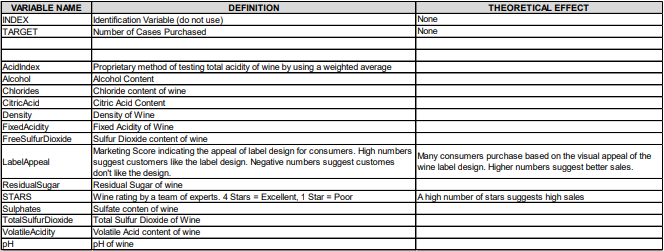
\includegraphics{https://raw.githubusercontent.com/djlofland/DS621_F2020_Group3/master/Homework_5/figures/Variables.png}
\caption{Variables of Interest}
\end{figure}

Given that the Index column had no impact on the target variable, number
of wines, it was dropped.

\hypertarget{summary-stats}{%
\subsubsection{Summary Stats}\label{summary-stats}}

We compiled summary statistics on our data set to better understand the
data before modeling.

\begin{verbatim}
##      TARGET       FixedAcidity     VolatileAcidity     CitricAcid     
##  Min.   :0.000   Min.   :-18.100   Min.   :-2.7900   Min.   :-3.2400  
##  1st Qu.:2.000   1st Qu.:  5.200   1st Qu.: 0.1300   1st Qu.: 0.0300  
##  Median :3.000   Median :  6.900   Median : 0.2800   Median : 0.3100  
##  Mean   :3.029   Mean   :  7.076   Mean   : 0.3241   Mean   : 0.3084  
##  3rd Qu.:4.000   3rd Qu.:  9.500   3rd Qu.: 0.6400   3rd Qu.: 0.5800  
##  Max.   :8.000   Max.   : 34.400   Max.   : 3.6800   Max.   : 3.8600  
##                                                                       
##  ResidualSugar        Chlorides       FreeSulfurDioxide TotalSulfurDioxide
##  Min.   :-127.800   Min.   :-1.1710   Min.   :-555.00   Min.   :-823.0    
##  1st Qu.:  -2.000   1st Qu.:-0.0310   1st Qu.:   0.00   1st Qu.:  27.0    
##  Median :   3.900   Median : 0.0460   Median :  30.00   Median : 123.0    
##  Mean   :   5.419   Mean   : 0.0548   Mean   :  30.85   Mean   : 120.7    
##  3rd Qu.:  15.900   3rd Qu.: 0.1530   3rd Qu.:  70.00   3rd Qu.: 208.0    
##  Max.   : 141.150   Max.   : 1.3510   Max.   : 623.00   Max.   :1057.0    
##  NA's   :616        NA's   :638       NA's   :647       NA's   :682       
##     Density             pH          Sulphates          Alcohol     
##  Min.   :0.8881   Min.   :0.480   Min.   :-3.1300   Min.   :-4.70  
##  1st Qu.:0.9877   1st Qu.:2.960   1st Qu.: 0.2800   1st Qu.: 9.00  
##  Median :0.9945   Median :3.200   Median : 0.5000   Median :10.40  
##  Mean   :0.9942   Mean   :3.208   Mean   : 0.5271   Mean   :10.49  
##  3rd Qu.:1.0005   3rd Qu.:3.470   3rd Qu.: 0.8600   3rd Qu.:12.40  
##  Max.   :1.0992   Max.   :6.130   Max.   : 4.2400   Max.   :26.50  
##                   NA's   :395     NA's   :1210      NA's   :653    
##   LabelAppeal          AcidIndex          STARS      
##  Min.   :-2.000000   Min.   : 4.000   Min.   :1.000  
##  1st Qu.:-1.000000   1st Qu.: 7.000   1st Qu.:1.000  
##  Median : 0.000000   Median : 8.000   Median :2.000  
##  Mean   :-0.009066   Mean   : 7.773   Mean   :2.042  
##  3rd Qu.: 1.000000   3rd Qu.: 8.000   3rd Qu.:3.000  
##  Max.   : 2.000000   Max.   :17.000   Max.   :4.000  
##                                       NA's   :3359
\end{verbatim}

The first observation is the prevalance of NA's throughout the dataset.
Of the 14 feature columns, 8 of them contain at least some NA values. We
also see that the \texttt{TARGET} value is always between 0 and 8, which
makes sense as this is the ``Number of Cases of Wine Sold'' (we would
not expect partial cases).

We also note that many of the numerical features measuring the quantity
of a chemical in the wine have a negative minimum value. We are assuming
the original chemical measurements were normalized (possible a log
transform) allowing for negative values, since technically negative
concentrations shouldn't be physically possible. As such, we chose to
leave those values as-is.

\hypertarget{distributions}{%
\subsubsection{Distributions}\label{distributions}}

Next, we wanted to get an idea of the distribution profiles for each of
the variables.

\includegraphics{Homework5_Group3_files/figure-latex/unnamed-chunk-4-1.pdf}

We see that most variables have a somewhat normal (although steep)
distribution.

The distribution profiles show right skew in variables
\texttt{AcidIndex}, and \texttt{STARS}.

More interesting is the shape of many features where they are centered
with most values clustered at the center and somewhat uniform shape
above and below. It almost appears like a tri-modal distribution with a
low, middle and high normal distributions overlapping. We are not going
to do extensive feature engineer, or we might consider breaking these
features up into 3 separate features each. Two approaches include:

\begin{enumerate}
\def\labelenumi{\arabic{enumi}.}
\tightlist
\item
  Use \texttt{mixTools} to separate the multi-modal curves into 3
  distinct (and separate) features each capturing just the \texttt{low},
  \texttt{middle} or \texttt{high} values and retaining a numerical
  value.
\item
  Discretize the features converting them into categorical values
  indicating \texttt{low}, \texttt{middle} or \texttt{high} value.
\end{enumerate}

\hypertarget{boxplots}{%
\subsubsection{Boxplots}\label{boxplots}}

In addition to creating histogram distributions, we also elected to use
box-plots to get an idea of the spread of each variable.

\includegraphics{Homework5_Group3_files/figure-latex/unnamed-chunk-5-1.pdf}

\includegraphics{Homework5_Group3_files/figure-latex/unnamed-chunk-6-1.pdf}

The box-plots do not reveal any enormous outliers in any of the
features, meaning it is unlikely we will need to perform outlier
detection and removal. \texttt{AcidIndex}, \texttt{LabelAppeal}, and
\texttt{STARS} are essentially categorical in nature (ordinal), so we
explore how each value of those features relates with \texttt{TARGET}.
We see a clear relationship - as \texttt{LabelAppeal} increases, so does
\texttt{TARGET}.

We see the same relationship between \texttt{STARS} and \texttt{TARGET}
- we especially note that \texttt{STARS=NA} highly correlates with lower
\texttt{TARGET}. In the original project instructions, attention was
drawn to the fact that missing data might be informative. Based on this,
we will impute \texttt{STARS=NA} into \texttt{STARS=0} which fits with
the other values we see for \texttt{STARS} and the pattern that as stars
increase, cases sold increase.

\hypertarget{variable-plots}{%
\subsubsection{Variable Plots}\label{variable-plots}}

Finally, we wanted to plot scatter plots of each variable versus the
target variable, TARGET, to get an idea of the relationship between
them.

\includegraphics{Homework5_Group3_files/figure-latex/unnamed-chunk-7-1.pdf}

Due to the discrete nature of the target, it is somewhat difficult to
see clear linear relationships in the data. However, it does appear that
both \texttt{STARS} and \texttt{LabelAppeal} have a significant positive
relationship with the \texttt{TARGET}, and many of the chemical features
have at least some negative relationship with the \texttt{TARGET} as
lower values led to more values of 8 and 7 in the target variable.

Overall, although our plots indicate some interesting relationships
between our variables, they also reveal some significant issues with the
data.

For instance, most of the predictor variables are skewed or non-normally
distributed, and will need to be transformed. Additionally, there are
many data points that contain missing data that will need to be either
imputed or discarded. There also was the issue of nonsensical negative
values. We have chosen to take the absolute value of these as the
feature value as there are so many of these values: however, there is no
evidence to back up that this is a correct decision and that these
values are not simply missing.

\hypertarget{missing-data}{%
\subsubsection{Missing Data}\label{missing-data}}

When we initially viewed the first few rows of the raw data, we already
noticed missing data. Let's assess which fields have missing data.

\begin{verbatim}
##    values                ind
## 1   26.25              STARS
## 2    9.46          Sulphates
## 3    5.33 TotalSulfurDioxide
## 4    5.10            Alcohol
## 5    5.06  FreeSulfurDioxide
## 6    4.99          Chlorides
## 7    4.81      ResidualSugar
## 8    3.09                 pH
## 9    0.00             TARGET
## 10   0.00       FixedAcidity
## 11   0.00    VolatileAcidity
## 12   0.00         CitricAcid
## 13   0.00            Density
## 14   0.00        LabelAppeal
## 15   0.00          AcidIndex
\end{verbatim}

In the project description, it was noted that the fact that a certain
variable is missing may be predictive. We will impute \texttt{STARS=NA}
to \texttt{STARS=0}. We will impute the remaining missing data using
\texttt{caret::preProcess} and \texttt{method=knnImpute}. Note that
\texttt{preProcess} will also center, scale and \texttt{BoxCox} our
features at the same time.

\hypertarget{feature-target-correlations}{%
\subsubsection{Feature-Target
Correlations}\label{feature-target-correlations}}

With our missing data imputed correctly, we can now build off the
scatter plots from above to quantify the correlations between our target
variable and predictor variable. We will want to choose those with
stronger positive or negative correlations. Features with correlations
closer to zero will probably not provide any meaningful information on
explaining wins by a team.

\begin{verbatim}
##          values                ind
## 1   0.685381473              STARS
## 2   0.356500469        LabelAppeal
## 3   0.062030498            Alcohol
## 4   0.051730323 TotalSulfurDioxide
## 5   0.043996542  FreeSulfurDioxide
## 6   0.016187709      ResidualSugar
## 7   0.008684633         CitricAcid
## 8  -0.009081197                 pH
## 9  -0.035589560            Density
## 10 -0.039072231          Chlorides
## 11 -0.039917146          Sulphates
## 12 -0.049010939       FixedAcidity
## 13 -0.088793212    VolatileAcidity
## 14 -0.221991949          AcidIndex
\end{verbatim}

\texttt{STARS}, \texttt{LabelAppeal}, and \texttt{Alcohol} have the
highest correlation with \texttt{TARGET}, which matches what we saw in
the variable plots above. Recall that we imputed \texttt{NA} values for
\texttt{STARS} as \texttt{0}. WE note that the missing value dummy
indicators do not correlate with \texttt{TARGET}, so these additional
columns may not provide much additional predictive power. We will
include them for now.

\hypertarget{multicolinearity}{%
\subsubsection{Multicolinearity}\label{multicolinearity}}

One problem that can occur with multi-variable regression is correlation
between variables, or multicolinearity. A quick check is to run
correlations between variables.

\includegraphics{Homework5_Group3_files/figure-latex/unnamed-chunk-11-1.pdf}

We see that the features have very low correlations with each other,
meaning that there is not much multicollinearity present in the dataset.
This means that the assumptions of linear regression are more likely to
be met.

\hypertarget{data-preparation}{%
\subsection{2. Data Preparation}\label{data-preparation}}

To summarize our data preparation and exploration, we can distinguish
our findings into a few categories below:

\hypertarget{removed-fields}{%
\subsubsection{Removed Fields}\label{removed-fields}}

We removed the INDEX field as it offers no information for a model.

\hypertarget{missing-values}{%
\subsubsection{Missing Values}\label{missing-values}}

For the 8 features with missing values, we created a dummy variable that
is 1 if the value is missing and 0 if it is not. We then imputed the
missing values as the median of the feature, allowing us to using
records with missing values while still including the information that
the value is missing.

\hypertarget{outliers}{%
\subsubsection{Outliers}\label{outliers}}

Many of the numerical features had unreasonable negative values. We
transformed these to be the absolute value of the feature, as a data
entry error seems likely given the quantity of negative records.

\hypertarget{transform-non-normal-variables}{%
\subsubsection{Transform non-normal
variables}\label{transform-non-normal-variables}}

Finally, as mentioned earlier in our data exploration, during the impute
step, \texttt{caret::preProcess()} automatically centered, scaled and
BoxCox transformed our data. Here are some plots to demonstrate the
changes in distributions and final values after the transformations:

\includegraphics{Homework5_Group3_files/figure-latex/unnamed-chunk-12-1.pdf}

We see that after the transformations, the variables are more centered
and more closely resemble a normal distribution, although clearly they
are still not perfect normal distributions.

\hypertarget{finalizing-the-dataset-for-model-building}{%
\subsubsection{Finalizing the dataset for model
building}\label{finalizing-the-dataset-for-model-building}}

With our transformations complete, we can now add these into our
\texttt{clean\_df} dataframe and continue on to build our models. To
better measure each model performance, we split our data into a training
and testing data set. We will train using the first, then measure model
performance again the testing hold out set.

\begin{verbatim}
## [1] "Number of Training Samples:  10238"
\end{verbatim}

\begin{verbatim}
## [1] "Number of Testing Samples:  2557"
\end{verbatim}

\hypertarget{model-building}{%
\subsection{3. Model Building}\label{model-building}}

\hypertarget{poisson-model-1}{%
\subsubsection{Poisson Model 1}\label{poisson-model-1}}

In this first model, we include all available features. Features
include:

\texttt{FixedAcidity}, \texttt{VolatileAcidity}, \texttt{CitricAcid},
\texttt{ResidualSugar}, \texttt{Chlorides}, \texttt{FreeSulfurDioxide},
\texttt{TotalSulfurDioxide}, \texttt{Density}, \texttt{pH},
\texttt{Sulphates}, \texttt{Alcohol}, \texttt{LabelAppeal},
\texttt{AcidIndex}, \texttt{STARS}

\begin{verbatim}
## 
## Call:
## glm(formula = TARGET ~ FixedAcidity + VolatileAcidity + CitricAcid + 
##     ResidualSugar + Chlorides + FreeSulfurDioxide + TotalSulfurDioxide + 
##     Density + pH + Sulphates + Alcohol + as.factor(LabelAppeal) + 
##     as.factor(AcidIndex) + as.factor(STARS), family = poisson, 
##     data = trainingData)
## 
## Deviance Residuals: 
##     Min       1Q   Median       3Q      Max  
## -3.2283  -0.6434  -0.0031   0.4448   3.4457  
## 
## Coefficients:
##                                             Estimate  Std. Error z value
## (Intercept)                                0.4439916   0.4495502   0.988
## FixedAcidity                               0.0040402   0.0058116   0.695
## VolatileAcidity                           -0.0234214   0.0057226  -4.093
## CitricAcid                                 0.0032509   0.0057015   0.570
## ResidualSugar                             -0.0000278   0.0058154  -0.005
## Chlorides                                 -0.0108552   0.0058652  -1.851
## FreeSulfurDioxide                          0.0140285   0.0057877   2.424
## TotalSulfurDioxide                         0.0197772   0.0058265   3.394
## Density                                   -0.0034164   0.0057167  -0.598
## pH                                        -0.0074096   0.0057465  -1.289
## Sulphates                                 -0.0082029   0.0059273  -1.384
## Alcohol                                    0.0155900   0.0058440   2.668
## as.factor(LabelAppeal)-1.11204793733397    0.2303607   0.0422310   5.455
## as.factor(LabelAppeal)0.0101741115806247   0.4176697   0.0412107  10.135
## as.factor(LabelAppeal)1.13239616049522     0.5597080   0.0419413  13.345
## as.factor(LabelAppeal)2.25461820940981     0.6850372   0.0471421  14.531
## as.factor(AcidIndex)-3.59682937695875     -0.5852519   0.4530978  -1.292
## as.factor(AcidIndex)-1.79176983045029     -0.5203594   0.4483464  -1.161
## as.factor(AcidIndex)-0.545318540973785    -0.5552133   0.4481201  -1.239
## as.factor(AcidIndex)0.362910765511677     -0.5867807   0.4481419  -1.309
## as.factor(AcidIndex)1.05172974217783      -0.7021374   0.4484237  -1.566
## as.factor(AcidIndex)1.59059728918163      -0.8280728   0.4493229  -1.843
## as.factor(AcidIndex)2.02271372429848      -1.2437196   0.4525965  -2.748
## as.factor(AcidIndex)2.37629509167962      -1.1958462   0.4567626  -2.618
## as.factor(AcidIndex)2.67051656830802      -1.1237704   0.4610222  -2.438
## as.factor(AcidIndex)2.9188445277671       -1.0988122   0.4704004  -2.336
## as.factor(AcidIndex)3.13100139587667      -0.6690141   0.5131206  -1.304
## as.factor(AcidIndex)3.31417429494859      -0.9267966   0.6333688  -1.463
## as.factor(AcidIndex)3.47378568897179     -13.2441367 126.8763094  -0.104
## as.factor(STARS)-0.42623524866846          0.7494810   0.0217868  34.401
## as.factor(STARS)0.416552574962037          1.0666709   0.0204008  52.286
## as.factor(STARS)1.25934039859254           1.1842232   0.0214239  55.276
## as.factor(STARS)2.10212822222303           1.3049938   0.0271484  48.069
##                                                      Pr(>|z|)    
## (Intercept)                                          0.323331    
## FixedAcidity                                         0.486931    
## VolatileAcidity                                   0.000042622 ***
## CitricAcid                                           0.568551    
## ResidualSugar                                        0.996185    
## Chlorides                                            0.064201 .  
## FreeSulfurDioxide                                    0.015357 *  
## TotalSulfurDioxide                                   0.000688 ***
## Density                                              0.550091    
## pH                                                   0.197258    
## Sulphates                                            0.166381    
## Alcohol                                              0.007637 ** 
## as.factor(LabelAppeal)-1.11204793733397           0.000000049 ***
## as.factor(LabelAppeal)0.0101741115806247 < 0.0000000000000002 ***
## as.factor(LabelAppeal)1.13239616049522   < 0.0000000000000002 ***
## as.factor(LabelAppeal)2.25461820940981   < 0.0000000000000002 ***
## as.factor(AcidIndex)-3.59682937695875                0.196472    
## as.factor(AcidIndex)-1.79176983045029                0.245797    
## as.factor(AcidIndex)-0.545318540973785               0.215352    
## as.factor(AcidIndex)0.362910765511677                0.190411    
## as.factor(AcidIndex)1.05172974217783                 0.117398    
## as.factor(AcidIndex)1.59059728918163                 0.065339 .  
## as.factor(AcidIndex)2.02271372429848                 0.005997 ** 
## as.factor(AcidIndex)2.37629509167962                 0.008842 ** 
## as.factor(AcidIndex)2.67051656830802                 0.014787 *  
## as.factor(AcidIndex)2.9188445277671                  0.019496 *  
## as.factor(AcidIndex)3.13100139587667                 0.192297    
## as.factor(AcidIndex)3.31417429494859                 0.143390    
## as.factor(AcidIndex)3.47378568897179                 0.916863    
## as.factor(STARS)-0.42623524866846        < 0.0000000000000002 ***
## as.factor(STARS)0.416552574962037        < 0.0000000000000002 ***
## as.factor(STARS)1.25934039859254         < 0.0000000000000002 ***
## as.factor(STARS)2.10212822222303         < 0.0000000000000002 ***
## ---
## Signif. codes:  0 '***' 0.001 '**' 0.01 '*' 0.05 '.' 0.1 ' ' 1
## 
## (Dispersion parameter for poisson family taken to be 1)
## 
##     Null deviance: 18210  on 10237  degrees of freedom
## Residual deviance: 10766  on 10205  degrees of freedom
## AIC: 36440
## 
## Number of Fisher Scoring iterations: 10
\end{verbatim}

\begin{verbatim}
##          RMSE      Rsquared           MAE           aic           bic 
##     2.6045113     0.4321849     2.2322328 36439.5803573 36678.2977890
\end{verbatim}

\hypertarget{poisson-model-2}{%
\subsubsection{Poisson Model 2}\label{poisson-model-2}}

In this second model, we only include the most predictive features based
on our first Poisson Model. The predictors for the following model are:

\texttt{VolatileAcidity}, \texttt{TotalSulfurDioxide}, \texttt{Alcohol},
\texttt{LabelAppeal}, \texttt{AcidIndex}, \texttt{STARS}

\begin{verbatim}
## 
## Call:
## glm(formula = TARGET ~ VolatileAcidity + TotalSulfurDioxide + 
##     Alcohol + as.factor(LabelAppeal) + as.factor(AcidIndex) + 
##     as.factor(STARS), family = poisson, data = clean_df)
## 
## Deviance Residuals: 
##     Min       1Q   Median       3Q      Max  
## -3.2335  -0.6501  -0.0035   0.4410   3.6951  
## 
## Coefficients:
##                                           Estimate Std. Error z value
## (Intercept)                               0.001201   0.318675   0.004
## VolatileAcidity                          -0.023533   0.005122  -4.595
## TotalSulfurDioxide                        0.016952   0.005244   3.232
## Alcohol                                   0.016009   0.005231   3.060
## as.factor(LabelAppeal)-1.11204793733397   0.240289   0.037999   6.324
## as.factor(LabelAppeal)0.0101741115806247  0.430806   0.037064  11.623
## as.factor(LabelAppeal)1.13239616049522    0.564104   0.037710  14.959
## as.factor(LabelAppeal)2.25461820940981    0.699216   0.042446  16.473
## as.factor(AcidIndex)-3.59682937695875    -0.140143   0.322337  -0.435
## as.factor(AcidIndex)-1.79176983045029    -0.097789   0.316887  -0.309
## as.factor(AcidIndex)-0.545318540973785   -0.131342   0.316605  -0.415
## as.factor(AcidIndex)0.362910765511677    -0.162635   0.316637  -0.514
## as.factor(AcidIndex)1.05172974217783     -0.272917   0.316940  -0.861
## as.factor(AcidIndex)1.59059728918163     -0.432064   0.318025  -1.359
## as.factor(AcidIndex)2.02271372429848     -0.795786   0.321596  -2.474
## as.factor(AcidIndex)2.37629509167962     -0.810861   0.327262  -2.478
## as.factor(AcidIndex)2.67051656830802     -0.646459   0.330156  -1.958
## as.factor(AcidIndex)2.9188445277671      -0.738613   0.342710  -2.155
## as.factor(AcidIndex)3.13100139587667     -0.286638   0.403433  -0.710
## as.factor(AcidIndex)3.31417429494859     -0.951704   0.547993  -1.737
## as.factor(AcidIndex)3.47378568897179     -1.196936   0.548071  -2.184
## as.factor(STARS)-0.42623524866846         0.757245   0.019564  38.705
## as.factor(STARS)0.416552574962037         1.075518   0.018261  58.896
## as.factor(STARS)1.25934039859254          1.194174   0.019232  62.093
## as.factor(STARS)2.10212822222303          1.313789   0.024330  53.999
##                                                      Pr(>|z|)    
## (Intercept)                                           0.99699    
## VolatileAcidity                                0.000004335408 ***
## TotalSulfurDioxide                                    0.00123 ** 
## Alcohol                                               0.00221 ** 
## as.factor(LabelAppeal)-1.11204793733397        0.000000000256 ***
## as.factor(LabelAppeal)0.0101741115806247 < 0.0000000000000002 ***
## as.factor(LabelAppeal)1.13239616049522   < 0.0000000000000002 ***
## as.factor(LabelAppeal)2.25461820940981   < 0.0000000000000002 ***
## as.factor(AcidIndex)-3.59682937695875                 0.66373    
## as.factor(AcidIndex)-1.79176983045029                 0.75763    
## as.factor(AcidIndex)-0.545318540973785                0.67825    
## as.factor(AcidIndex)0.362910765511677                 0.60751    
## as.factor(AcidIndex)1.05172974217783                  0.38918    
## as.factor(AcidIndex)1.59059728918163                  0.17428    
## as.factor(AcidIndex)2.02271372429848                  0.01334 *  
## as.factor(AcidIndex)2.37629509167962                  0.01322 *  
## as.factor(AcidIndex)2.67051656830802                  0.05023 .  
## as.factor(AcidIndex)2.9188445277671                   0.03114 *  
## as.factor(AcidIndex)3.13100139587667                  0.47740    
## as.factor(AcidIndex)3.31417429494859                  0.08244 .  
## as.factor(AcidIndex)3.47378568897179                  0.02897 *  
## as.factor(STARS)-0.42623524866846        < 0.0000000000000002 ***
## as.factor(STARS)0.416552574962037        < 0.0000000000000002 ***
## as.factor(STARS)1.25934039859254         < 0.0000000000000002 ***
## as.factor(STARS)2.10212822222303         < 0.0000000000000002 ***
## ---
## Signif. codes:  0 '***' 0.001 '**' 0.01 '*' 0.05 '.' 0.1 ' ' 1
## 
## (Dispersion parameter for poisson family taken to be 1)
## 
##     Null deviance: 22861  on 12794  degrees of freedom
## Residual deviance: 13550  on 12770  degrees of freedom
## AIC: 45542
## 
## Number of Fisher Scoring iterations: 6
\end{verbatim}

\begin{verbatim}
##          RMSE      Rsquared           MAE           aic           bic 
##     2.5926126     0.5207382     2.2281793 45542.3183589 45728.7386026
\end{verbatim}

\hypertarget{negative-binomial-model-3}{%
\subsubsection{Negative Binomial Model
3}\label{negative-binomial-model-3}}

Similar to Poisson Model 1, the predictors for the following model are:

\texttt{FixedAcidity}, \texttt{VolatileAcidity}, \texttt{CitricAcid},
\texttt{ResidualSugar}, \texttt{Chlorides}, \texttt{FreeSulfurDioxide},
\texttt{TotalSulfurDioxide}, \texttt{Density}, \texttt{pH},
\texttt{Sulphates}, \texttt{Alcohol}, \texttt{LabelAppeal},
\texttt{AcidIndex}, \texttt{STARS}

\begin{verbatim}
## 
## Call:
## glm.nb(formula = TARGET ~ FixedAcidity + VolatileAcidity + CitricAcid + 
##     ResidualSugar + Chlorides + FreeSulfurDioxide + TotalSulfurDioxide + 
##     Density + pH + Sulphates + Alcohol + as.factor(LabelAppeal) + 
##     as.factor(AcidIndex) + as.factor(STARS), data = clean_df, 
##     init.theta = 40957.00343, link = log)
## 
## Deviance Residuals: 
##     Min       1Q   Median       3Q      Max  
## -3.2219  -0.6496  -0.0055   0.4446   3.6790  
## 
## Coefficients:
##                                            Estimate Std. Error z value
## (Intercept)                               0.0275198  0.3190721   0.086
## FixedAcidity                              0.0010176  0.0051829   0.196
## VolatileAcidity                          -0.0231944  0.0051231  -4.527
## CitricAcid                                0.0039724  0.0050838   0.781
## ResidualSugar                             0.0005767  0.0052060   0.111
## Chlorides                                -0.0122552  0.0052206  -2.347
## FreeSulfurDioxide                         0.0132531  0.0051832   2.557
## TotalSulfurDioxide                        0.0170166  0.0052484   3.242
## Density                                  -0.0074549  0.0050938  -1.464
## pH                                       -0.0066655  0.0051875  -1.285
## Sulphates                                -0.0106282  0.0053149  -2.000
## Alcohol                                   0.0157805  0.0052355   3.014
## as.factor(LabelAppeal)-1.11204793733397   0.2398534  0.0380017   6.312
## as.factor(LabelAppeal)0.0101741115806247  0.4300463  0.0370666  11.602
## as.factor(LabelAppeal)1.13239616049522    0.5633460  0.0377142  14.937
## as.factor(LabelAppeal)2.25461820940981    0.6992610  0.0424548  16.471
## as.factor(AcidIndex)-3.59682937695875    -0.1651538  0.3226593  -0.512
## as.factor(AcidIndex)-1.79176983045029    -0.1214774  0.3172467  -0.383
## as.factor(AcidIndex)-0.545318540973785   -0.1558113  0.3169954  -0.492
## as.factor(AcidIndex)0.362910765511677    -0.1871144  0.3170413  -0.590
## as.factor(AcidIndex)1.05172974217783     -0.2972766  0.3173791  -0.937
## as.factor(AcidIndex)1.59059728918163     -0.4542592  0.3184811  -1.426
## as.factor(AcidIndex)2.02271372429848     -0.8158352  0.3220684  -2.533
## as.factor(AcidIndex)2.37629509167962     -0.8303961  0.3277299  -2.534
## as.factor(AcidIndex)2.67051656830802     -0.6688133  0.3306330  -2.023
## as.factor(AcidIndex)2.9188445277671      -0.7687131  0.3432641  -2.239
## as.factor(AcidIndex)3.13100139587667     -0.3297889  0.4038365  -0.817
## as.factor(AcidIndex)3.31417429494859     -0.9814037  0.5484760  -1.789
## as.factor(AcidIndex)3.47378568897179     -1.2022430  0.5486104  -2.191
## as.factor(STARS)-0.42623524866846         0.7548590  0.0195728  38.567
## as.factor(STARS)0.416552574962037         1.0732229  0.0182738  58.730
## as.factor(STARS)1.25934039859254          1.1910222  0.0192473  61.880
## as.factor(STARS)2.10212822222303          1.3117031  0.0243440  53.882
##                                                      Pr(>|z|)    
## (Intercept)                                           0.93127    
## FixedAcidity                                          0.84435    
## VolatileAcidity                                0.000005971523 ***
## CitricAcid                                            0.43458    
## ResidualSugar                                         0.91179    
## Chlorides                                             0.01890 *  
## FreeSulfurDioxide                                     0.01056 *  
## TotalSulfurDioxide                                    0.00119 ** 
## Density                                               0.14332    
## pH                                                    0.19882    
## Sulphates                                             0.04554 *  
## Alcohol                                               0.00258 ** 
## as.factor(LabelAppeal)-1.11204793733397        0.000000000276 ***
## as.factor(LabelAppeal)0.0101741115806247 < 0.0000000000000002 ***
## as.factor(LabelAppeal)1.13239616049522   < 0.0000000000000002 ***
## as.factor(LabelAppeal)2.25461820940981   < 0.0000000000000002 ***
## as.factor(AcidIndex)-3.59682937695875                 0.60875    
## as.factor(AcidIndex)-1.79176983045029                 0.70179    
## as.factor(AcidIndex)-0.545318540973785                0.62305    
## as.factor(AcidIndex)0.362910765511677                 0.55506    
## as.factor(AcidIndex)1.05172974217783                  0.34893    
## as.factor(AcidIndex)1.59059728918163                  0.15377    
## as.factor(AcidIndex)2.02271372429848                  0.01131 *  
## as.factor(AcidIndex)2.37629509167962                  0.01128 *  
## as.factor(AcidIndex)2.67051656830802                  0.04309 *  
## as.factor(AcidIndex)2.9188445277671                   0.02513 *  
## as.factor(AcidIndex)3.13100139587667                  0.41413    
## as.factor(AcidIndex)3.31417429494859                  0.07356 .  
## as.factor(AcidIndex)3.47378568897179                  0.02842 *  
## as.factor(STARS)-0.42623524866846        < 0.0000000000000002 ***
## as.factor(STARS)0.416552574962037        < 0.0000000000000002 ***
## as.factor(STARS)1.25934039859254         < 0.0000000000000002 ***
## as.factor(STARS)2.10212822222303         < 0.0000000000000002 ***
## ---
## Signif. codes:  0 '***' 0.001 '**' 0.01 '*' 0.05 '.' 0.1 ' ' 1
## 
## (Dispersion parameter for Negative Binomial(40957) family taken to be 1)
## 
##     Null deviance: 22860  on 12794  degrees of freedom
## Residual deviance: 13529  on 12762  degrees of freedom
## AIC: 45540
## 
## Number of Fisher Scoring iterations: 1
## 
## 
##               Theta:  40957 
##           Std. Err.:  34344 
## Warning while fitting theta: iteration limit reached 
## 
##  2 x log-likelihood:  -45472.13
\end{verbatim}

\begin{verbatim}
##          RMSE      Rsquared           MAE           aic           bic 
##     2.5923418     0.5217514     2.2278411 45540.1321542 45793.6636857
\end{verbatim}

\hypertarget{negative-binomial-model-4}{%
\subsubsection{Negative Binomial Model
4}\label{negative-binomial-model-4}}

Similar to Poisson Model 2, the predictors for the following model are:

\texttt{VolatileAcidity}, \texttt{FreeSulfurDioxide},
\texttt{TotalSulfurDioxide}, \texttt{Alcohol}, \texttt{LabelAppeal},
\texttt{AcidIndex}, \texttt{STARS}

\begin{verbatim}
## 
## Call:
## glm.nb(formula = TARGET ~ VolatileAcidity + FreeSulfurDioxide + 
##     TotalSulfurDioxide + Alcohol + as.factor(LabelAppeal) + as.factor(AcidIndex) + 
##     as.factor(STARS), data = clean_df, init.theta = 40912.68498, 
##     link = log)
## 
## Deviance Residuals: 
##     Min       1Q   Median       3Q      Max  
## -3.2456  -0.6517  -0.0038   0.4399   3.6952  
## 
## Coefficients:
##                                           Estimate Std. Error z value
## (Intercept)                               0.014317   0.318731   0.045
## VolatileAcidity                          -0.023451   0.005122  -4.578
## FreeSulfurDioxide                         0.013266   0.005179   2.562
## TotalSulfurDioxide                        0.016879   0.005244   3.219
## Alcohol                                   0.016237   0.005231   3.104
## as.factor(LabelAppeal)-1.11204793733397   0.240039   0.038000   6.317
## as.factor(LabelAppeal)0.0101741115806247  0.430314   0.037065  11.610
## as.factor(LabelAppeal)1.13239616049522    0.563287   0.037712  14.936
## as.factor(LabelAppeal)2.25461820940981    0.698162   0.042449  16.447
## as.factor(AcidIndex)-3.59682937695875    -0.154135   0.322401  -0.478
## as.factor(AcidIndex)-1.79176983045029    -0.110580   0.316945  -0.349
## as.factor(AcidIndex)-0.545318540973785   -0.143771   0.316660  -0.454
## as.factor(AcidIndex)0.362910765511677    -0.174856   0.316690  -0.552
## as.factor(AcidIndex)1.05172974217783     -0.285228   0.316994  -0.900
## as.factor(AcidIndex)1.59059728918163     -0.443142   0.318072  -1.393
## as.factor(AcidIndex)2.02271372429848     -0.806122   0.321638  -2.506
## as.factor(AcidIndex)2.37629509167962     -0.819576   0.327296  -2.504
## as.factor(AcidIndex)2.67051656830802     -0.655682   0.330193  -1.986
## as.factor(AcidIndex)2.9188445277671      -0.753474   0.342775  -2.198
## as.factor(AcidIndex)3.13100139587667     -0.299583   0.403483  -0.742
## as.factor(AcidIndex)3.31417429494859     -0.953685   0.548008  -1.740
## as.factor(AcidIndex)3.47378568897179     -1.205542   0.548094  -2.200
## as.factor(STARS)-0.42623524866846         0.756497   0.019567  38.662
## as.factor(STARS)0.416552574962037         1.074730   0.018264  58.844
## as.factor(STARS)1.25934039859254          1.193602   0.019234  62.057
## as.factor(STARS)2.10212822222303          1.314420   0.024331  54.023
##                                                      Pr(>|z|)    
## (Intercept)                                           0.96417    
## VolatileAcidity                                0.000004685011 ***
## FreeSulfurDioxide                                     0.01042 *  
## TotalSulfurDioxide                                    0.00129 ** 
## Alcohol                                               0.00191 ** 
## as.factor(LabelAppeal)-1.11204793733397        0.000000000267 ***
## as.factor(LabelAppeal)0.0101741115806247 < 0.0000000000000002 ***
## as.factor(LabelAppeal)1.13239616049522   < 0.0000000000000002 ***
## as.factor(LabelAppeal)2.25461820940981   < 0.0000000000000002 ***
## as.factor(AcidIndex)-3.59682937695875                 0.63259    
## as.factor(AcidIndex)-1.79176983045029                 0.72717    
## as.factor(AcidIndex)-0.545318540973785                0.64981    
## as.factor(AcidIndex)0.362910765511677                 0.58086    
## as.factor(AcidIndex)1.05172974217783                  0.36823    
## as.factor(AcidIndex)1.59059728918163                  0.16356    
## as.factor(AcidIndex)2.02271372429848                  0.01220 *  
## as.factor(AcidIndex)2.37629509167962                  0.01228 *  
## as.factor(AcidIndex)2.67051656830802                  0.04706 *  
## as.factor(AcidIndex)2.9188445277671                   0.02794 *  
## as.factor(AcidIndex)3.13100139587667                  0.45779    
## as.factor(AcidIndex)3.31417429494859                  0.08181 .  
## as.factor(AcidIndex)3.47378568897179                  0.02784 *  
## as.factor(STARS)-0.42623524866846        < 0.0000000000000002 ***
## as.factor(STARS)0.416552574962037        < 0.0000000000000002 ***
## as.factor(STARS)1.25934039859254         < 0.0000000000000002 ***
## as.factor(STARS)2.10212822222303         < 0.0000000000000002 ***
## ---
## Signif. codes:  0 '***' 0.001 '**' 0.01 '*' 0.05 '.' 0.1 ' ' 1
## 
## (Dispersion parameter for Negative Binomial(40912.68) family taken to be 1)
## 
##     Null deviance: 22860  on 12794  degrees of freedom
## Residual deviance: 13543  on 12769  degrees of freedom
## AIC: 45540
## 
## Number of Fisher Scoring iterations: 1
## 
## 
##               Theta:  40913 
##           Std. Err.:  34297 
## Warning while fitting theta: iteration limit reached 
## 
##  2 x log-likelihood:  -45486.18
\end{verbatim}

\begin{verbatim}
##          RMSE      Rsquared           MAE           aic           bic 
##     2.5924956     0.5211834     2.2280509 45540.1774651 45741.5113283
\end{verbatim}

\hypertarget{linear-model-5}{%
\subsubsection{Linear Model 5}\label{linear-model-5}}

The predictors for the following model are:

\texttt{FixedAcidity}, \texttt{VolatileAcidity}, \texttt{CitricAcid},
\texttt{ResidualSugar}, \texttt{Chlorides}, \texttt{FreeSulfurDioxide},
\texttt{TotalSulfurDioxide}, \texttt{Density}, \texttt{pH},
\texttt{Sulphates}, \texttt{Alcohol}, \texttt{LabelAppeal},
\texttt{AcidIndex}, \texttt{STARS}

\begin{verbatim}
## 
## Call:
## lm(formula = TARGET ~ FixedAcidity + VolatileAcidity + CitricAcid + 
##     ResidualSugar + Chlorides + FreeSulfurDioxide + TotalSulfurDioxide + 
##     Density + pH + Sulphates + Alcohol + as.factor(LabelAppeal) + 
##     as.factor(AcidIndex) + as.factor(STARS), data = clean_df)
## 
## Residuals:
##     Min      1Q  Median      3Q     Max 
## -4.9635 -0.8591  0.0325  0.8384  6.0750 
## 
## Coefficients:
##                                           Estimate Std. Error t value
## (Intercept)                               0.995095   0.755491   1.317
## FixedAcidity                              0.004930   0.011720   0.421
## VolatileAcidity                          -0.073667   0.011565  -6.370
## CitricAcid                                0.014455   0.011558   1.251
## ResidualSugar                             0.004027   0.011782   0.342
## Chlorides                                -0.038485   0.011776  -3.268
## FreeSulfurDioxide                         0.039825   0.011786   3.379
## TotalSulfurDioxide                        0.049447   0.011816   4.185
## Density                                  -0.022475   0.011545  -1.947
## pH                                       -0.018619   0.011704  -1.591
## Sulphates                                -0.028248   0.012015  -2.351
## Alcohol                                   0.050812   0.011830   4.295
## as.factor(LabelAppeal)-1.11204793733397   0.367639   0.062729   5.861
## as.factor(LabelAppeal)0.0101741115806247  0.835185   0.061168  13.654
## as.factor(LabelAppeal)1.13239616049522    1.302062   0.063917  20.371
## as.factor(LabelAppeal)2.25461820940981    1.889951   0.084169  22.454
## as.factor(AcidIndex)-3.59682937695875    -0.334854   0.767938  -0.436
## as.factor(AcidIndex)-1.79176983045029    -0.220221   0.754101  -0.292
## as.factor(AcidIndex)-0.545318540973785   -0.322349   0.753472  -0.428
## as.factor(AcidIndex)0.362910765511677    -0.429363   0.753539  -0.570
## as.factor(AcidIndex)1.05172974217783     -0.732560   0.754117  -0.971
## as.factor(AcidIndex)1.59059728918163     -1.041297   0.755385  -1.378
## as.factor(AcidIndex)2.02271372429848     -1.513113   0.757752  -1.997
## as.factor(AcidIndex)2.37629509167962     -1.533481   0.762156  -2.012
## as.factor(AcidIndex)2.67051656830802     -1.552014   0.769606  -2.017
## as.factor(AcidIndex)2.9188445277671      -1.400154   0.777299  -1.801
## as.factor(AcidIndex)3.13100139587667     -0.692206   0.883131  -0.784
## as.factor(AcidIndex)3.31417429494859     -1.772148   0.952843  -1.860
## as.factor(AcidIndex)3.47378568897179     -1.920432   0.900840  -2.132
## as.factor(STARS)-0.42623524866846         1.346560   0.032920  40.904
## as.factor(STARS)0.416552574962037         2.381720   0.032021  74.381
## as.factor(STARS)1.25934039859254          2.942287   0.037079  79.352
## as.factor(STARS)2.10212822222303          3.629958   0.059150  61.368
##                                                      Pr(>|t|)    
## (Intercept)                                           0.18781    
## FixedAcidity                                          0.67401    
## VolatileAcidity                                0.000000000196 ***
## CitricAcid                                            0.21109    
## ResidualSugar                                         0.73251    
## Chlorides                                             0.00109 ** 
## FreeSulfurDioxide                                     0.00073 ***
## TotalSulfurDioxide                             0.000028712970 ***
## Density                                               0.05160 .  
## pH                                                    0.11167    
## Sulphates                                             0.01873 *  
## Alcohol                                        0.000017590098 ***
## as.factor(LabelAppeal)-1.11204793733397        0.000000004722 ***
## as.factor(LabelAppeal)0.0101741115806247 < 0.0000000000000002 ***
## as.factor(LabelAppeal)1.13239616049522   < 0.0000000000000002 ***
## as.factor(LabelAppeal)2.25461820940981   < 0.0000000000000002 ***
## as.factor(AcidIndex)-3.59682937695875                 0.66281    
## as.factor(AcidIndex)-1.79176983045029                 0.77027    
## as.factor(AcidIndex)-0.545318540973785                0.66879    
## as.factor(AcidIndex)0.362910765511677                 0.56883    
## as.factor(AcidIndex)1.05172974217783                  0.33136    
## as.factor(AcidIndex)1.59059728918163                  0.16807    
## as.factor(AcidIndex)2.02271372429848                  0.04586 *  
## as.factor(AcidIndex)2.37629509167962                  0.04424 *  
## as.factor(AcidIndex)2.67051656830802                  0.04375 *  
## as.factor(AcidIndex)2.9188445277671                   0.07168 .  
## as.factor(AcidIndex)3.13100139587667                  0.43317    
## as.factor(AcidIndex)3.31417429494859                  0.06293 .  
## as.factor(AcidIndex)3.47378568897179                  0.03304 *  
## as.factor(STARS)-0.42623524866846        < 0.0000000000000002 ***
## as.factor(STARS)0.416552574962037        < 0.0000000000000002 ***
## as.factor(STARS)1.25934039859254         < 0.0000000000000002 ***
## as.factor(STARS)2.10212822222303         < 0.0000000000000002 ***
## ---
## Signif. codes:  0 '***' 0.001 '**' 0.01 '*' 0.05 '.' 0.1 ' ' 1
## 
## Residual standard error: 1.302 on 12762 degrees of freedom
## Multiple R-squared:  0.5441, Adjusted R-squared:  0.5429 
## F-statistic: 475.9 on 32 and 12762 DF,  p-value: < 0.00000000000000022
\end{verbatim}

\begin{verbatim}
##          RMSE      Rsquared           MAE           aic           bic 
##     1.2981486     0.5451111     1.0176919 43106.3022739 43359.8338054
\end{verbatim}

\hypertarget{linear-model-6}{%
\subsubsection{Linear Model 6}\label{linear-model-6}}

For the final Linear Model, we leverage \texttt{stepAIC} on our Linear
Model \#5 to choose the most important features.

\begin{verbatim}
## 
## Call:
## lm(formula = TARGET ~ VolatileAcidity + Chlorides + FreeSulfurDioxide + 
##     TotalSulfurDioxide + Density + pH + Sulphates + Alcohol + 
##     as.factor(LabelAppeal) + as.factor(AcidIndex) + as.factor(STARS), 
##     data = clean_df)
## 
## Residuals:
##     Min      1Q  Median      3Q     Max 
## -4.9616 -0.8590  0.0352  0.8399  6.0675 
## 
## Coefficients:
##                                          Estimate Std. Error t value
## (Intercept)                               0.99019    0.75488   1.312
## VolatileAcidity                          -0.07393    0.01156  -6.394
## Chlorides                                -0.03864    0.01177  -3.282
## FreeSulfurDioxide                         0.04009    0.01178   3.403
## TotalSulfurDioxide                        0.04960    0.01181   4.200
## Density                                  -0.02270    0.01154  -1.967
## pH                                       -0.01862    0.01170  -1.591
## Sulphates                                -0.02837    0.01201  -2.362
## Alcohol                                   0.05100    0.01183   4.313
## as.factor(LabelAppeal)-1.11204793733397   0.36722    0.06272   5.854
## as.factor(LabelAppeal)0.0101741115806247  0.83483    0.06116  13.649
## as.factor(LabelAppeal)1.13239616049522    1.30161    0.06391  20.367
## as.factor(LabelAppeal)2.25461820940981    1.88998    0.08416  22.456
## as.factor(AcidIndex)-3.59682937695875    -0.33511    0.76744  -0.437
## as.factor(AcidIndex)-1.79176983045029    -0.21824    0.75353  -0.290
## as.factor(AcidIndex)-0.545318540973785   -0.31837    0.75287  -0.423
## as.factor(AcidIndex)0.362910765511677    -0.42442    0.75293  -0.564
## as.factor(AcidIndex)1.05172974217783     -0.72561    0.75343  -0.963
## as.factor(AcidIndex)1.59059728918163     -1.03390    0.75463  -1.370
## as.factor(AcidIndex)2.02271372429848     -1.50407    0.75695  -1.987
## as.factor(AcidIndex)2.37629509167962     -1.52217    0.76131  -1.999
## as.factor(AcidIndex)2.67051656830802     -1.54018    0.76867  -2.004
## as.factor(AcidIndex)2.9188445277671      -1.38512    0.77635  -1.784
## as.factor(AcidIndex)3.13100139587667     -0.67937    0.88243  -0.770
## as.factor(AcidIndex)3.31417429494859     -1.75343    0.95178  -1.842
## as.factor(AcidIndex)3.47378568897179     -1.89498    0.89978  -2.106
## as.factor(STARS)-0.42623524866846         1.34682    0.03291  40.918
## as.factor(STARS)0.416552574962037         2.38256    0.03201  74.442
## as.factor(STARS)1.25934039859254          2.94276    0.03707  79.374
## as.factor(STARS)2.10212822222303          3.63105    0.05914  61.397
##                                                      Pr(>|t|)    
## (Intercept)                                          0.189639    
## VolatileAcidity                                0.000000000167 ***
## Chlorides                                            0.001034 ** 
## FreeSulfurDioxide                                    0.000669 ***
## TotalSulfurDioxide                             0.000026926678 ***
## Density                                              0.049224 *  
## pH                                                   0.111585    
## Sulphates                                            0.018191 *  
## Alcohol                                        0.000016245384 ***
## as.factor(LabelAppeal)-1.11204793733397        0.000000004904 ***
## as.factor(LabelAppeal)0.0101741115806247 < 0.0000000000000002 ***
## as.factor(LabelAppeal)1.13239616049522   < 0.0000000000000002 ***
## as.factor(LabelAppeal)2.25461820940981   < 0.0000000000000002 ***
## as.factor(AcidIndex)-3.59682937695875                0.662366    
## as.factor(AcidIndex)-1.79176983045029                0.772104    
## as.factor(AcidIndex)-0.545318540973785               0.672396    
## as.factor(AcidIndex)0.362910765511677                0.572976    
## as.factor(AcidIndex)1.05172974217783                 0.335525    
## as.factor(AcidIndex)1.59059728918163                 0.170687    
## as.factor(AcidIndex)2.02271372429848                 0.046941 *  
## as.factor(AcidIndex)2.37629509167962                 0.045584 *  
## as.factor(AcidIndex)2.67051656830802                 0.045124 *  
## as.factor(AcidIndex)2.9188445277671                  0.074426 .  
## as.factor(AcidIndex)3.13100139587667                 0.441383    
## as.factor(AcidIndex)3.31417429494859                 0.065461 .  
## as.factor(AcidIndex)3.47378568897179                 0.035220 *  
## as.factor(STARS)-0.42623524866846        < 0.0000000000000002 ***
## as.factor(STARS)0.416552574962037        < 0.0000000000000002 ***
## as.factor(STARS)1.25934039859254         < 0.0000000000000002 ***
## as.factor(STARS)2.10212822222303         < 0.0000000000000002 ***
## ---
## Signif. codes:  0 '***' 0.001 '**' 0.01 '*' 0.05 '.' 0.1 ' ' 1
## 
## Residual standard error: 1.302 on 12765 degrees of freedom
## Multiple R-squared:  0.544,  Adjusted R-squared:  0.543 
## F-statistic: 525.1 on 29 and 12765 DF,  p-value: < 0.00000000000000022
\end{verbatim}

\begin{verbatim}
##          RMSE      Rsquared           MAE           aic           bic 
##     1.2982178     0.5450624     1.0178541 43102.1597330 43333.3208352
\end{verbatim}

\hypertarget{model-selection-analysis}{%
\subsection{4. Model Selection \&
Analysis}\label{model-selection-analysis}}

This table summarizes the \textbf{RMSE}, \textbf{\(R^2\)}, \textbf{MAE},
\textbf{AIC} and \textbf{BIC} for all 6 models. In terms of raw metrics,
The Linear regressions (\textbf{Linear Model 5} and \textbf{Linear Model
6}) had the overall best performance based on \textbf{RMSE} and
\textbf{\(R^2\)}; however, \textbf{Poisson Model 1} had the best
performance based on \textbf{AIC} and \textbf{BIC}.

Overall, \textbf{RMSE} an \textbf{\(R^2\)} were not largely different
across the 6 models, given this we chose \textbf{Poisson Model 1} as our
final model since it had a far lower \textbf{AIC}.

\begin{table}[H]
\centering
\begin{tabular}{l|r|r|r|r|r}
\hline
  & RMSE & Rsquared & MAE & aic & bic\\
\hline
poiss1\_eval & 2.604511 & 0.4321849 & 2.232233 & 36439.58 & 36678.30\\
\hline
poiss2\_eval & 2.592613 & 0.5207382 & 2.228179 & 45542.32 & 45728.74\\
\hline
nb3\_eval & 2.592342 & 0.5217514 & 2.227841 & 45540.13 & 45793.66\\
\hline
nb4\_eval & 2.592496 & 0.5211834 & 2.228051 & 45540.18 & 45741.51\\
\hline
lm5\_eval & 1.298149 & 0.5451111 & 1.017692 & 43106.30 & 43359.83\\
\hline
lm6\_eval & 1.298218 & 0.5450624 & 1.017854 & 43102.16 & 43333.32\\
\hline
\end{tabular}
\end{table}

The final thing we will take a look at is our variable importance for
each model.

The final figure presented below shows the feature importance in each
model. As we see, all 6 models identified the same top 10 features.

\includegraphics{Homework5_Group3_files/figure-latex/unnamed-chunk-21-1.pdf}

\hypertarget{predictions}{%
\subsection{Predictions}\label{predictions}}

We apply \textbf{Poisson Model \#1} to the holdout evaluation set to
predict the \texttt{TARGET} for these instances. We have saved these
predictions as csv in the file \texttt{eval\_predictions.csv}.

Source code:
\url{https://github.com/djlofland/DS621_F2020_Group3/tree/master/Homework_5/eval_predictions.csv}

\begin{verbatim}
##      TARGET FixedAcidity VolatileAcidity  CitricAcid ResidualSugar   Chlorides
## 1 0.1977866  -0.26524401     -1.51030924 -0.04455813    -0.4776009  0.11673887
## 2 1.3734929   0.84276407      0.07767213 -1.23934313    -0.7442725  3.49856180
## 3 0.9436291   0.01967235      1.81871194 -0.16055667    -1.1383538  0.03195779
## 4 0.8554209  -0.13861451     -0.28584168  1.73021959    -0.1309278 -0.73421194
## 5 0.0224026   0.68447720     -0.14553811 -0.03295827    -0.1250018 -0.05282329
## 6 1.7062831   1.66585579     -0.36237090 -1.69173745    -0.1190758  1.50777652
##   FreeSulfurDioxide TotalSulfurDioxide    Density          pH  Sulphates
## 1       -0.05275591         1.19564455 -0.3402128  2.66647966  0.1211079
## 2       -0.45621338        -0.22730155 -0.1442311  0.23889195  0.6038736
## 3       -0.14689598        -0.19280589  1.9789246  2.06326090  0.1640204
## 4        0.49191169        -0.13675044 -0.2085894 -0.01122314  1.6981424
## 5        0.26328578        -0.29198092  1.3139028 -0.98225823 -0.6405890
## 6       -1.88848742         0.08315942 -1.6483055 -0.21720028 -0.5869484
##      Alcohol LabelAppeal  AcidIndex      STARS
## 1  0.4857435 -1.11204794 -1.7917698 -1.2690231
## 2  1.4782809  0.01017411 -1.7917698  0.4165526
## 3 -0.5202067  0.01017411  0.3629108 -0.4262352
## 4  0.4857435 -1.11204794  0.3629108 -0.4262352
## 5 -1.5261568  0.01017411  1.5905973 -1.2690231
## 6  0.2443154  1.13239616  0.3629108  2.1021282
\end{verbatim}

\hypertarget{references}{%
\subsection{References}\label{references}}

\begin{itemize}
\tightlist
\item
  A Modern Approach to Regression with R: Simon Sheather
\item
  Linear Models with R: Julian Faraway.
\item
  R package vignette,
  \href{https://cran.r-project.org/web/packages/mixtools/vignettes/mixtools.pdf}{mixtools:
  An R Package for Analyzing Finite Mixture Models}
\item
  \href{https://statisticsbyjim.com/regression/ols-linear-regression-assumptions/}{7
  Classic OLS assumptions}
\item
  \href{https://online.stat.psu.edu/stat462/node/180/}{Detecting
  Multicolinearity with VIF}
\end{itemize}

\hypertarget{appendix}{%
\subsection{Appendix}\label{appendix}}

\hypertarget{r-code}{%
\subsubsection{R Code}\label{r-code}}

\begin{verbatim}
# =====================================================================================
# Load Libraries and Define Helper functions 
# =====================================================================================

library(MASS)
library(rpart.plot)
library(ggplot2)
library(ggfortify)
library(gridExtra)
library(forecast)
library(fpp2)
library(fma)
library(kableExtra)
library(e1071)
library(mlbench)
library(ggcorrplot)
library(DataExplorer)
library(timeDate)
library(caret)
library(GGally)
library(corrplot)
library(RColorBrewer)
library(tibble)
library(tidyr)
library(tidyverse)
library(dplyr)
library(reshape2)
library(mixtools)
library(tidymodels)
library(ggpmisc)
library(regclass)
library(skimr)

#' Print a side-by-side Histogram and QQPlot of Residuals
#'
#' @param model A model
#' @examples
#' residPlot(myModel)
#' @return null
#' @export
residPlot <- function(model) {
  # Make sure a model was passed
  if (is.null(model)) {
    return
  }
  
  layout(matrix(c(1,1,2,3), 2, 2, byrow = TRUE))
  plot(residuals(model))
  hist(model[["residuals"]], freq = FALSE, breaks = "fd", main = "Residual Histogram",
       xlab = "Residuals",col="lightgreen")
  lines(density(model[["residuals"]], kernel = "ep"),col="blue", lwd=3)
  curve(dnorm(x,mean=mean(model[["residuals"]]), sd=sd(model[["residuals"]])), col="red", lwd=3, lty="dotted", add=T)
  qqnorm(model[["residuals"]], main = "Residual Q-Q plot")
  qqline(model[["residuals"]],col="red", lwd=3, lty="dotted")
  par(mfrow = c(1, 1))
}
#' Print a Variable Importance Plot for the provided model
#'
#' @param model The model
#' @param chart_title The Title to show on the plot
#' @examples
#' variableImportancePlot(myLinearModel, 'My Title)
#' @return null
#' @export
variableImportancePlot <- function(model=NULL, chart_title='Variable Importance Plot') {
  # Make sure a model was passed
  if (is.null(model)) {
    return
  }
  
  # use caret and gglot to print a variable importance plot
  varImp(model) %>% as.data.frame() %>% 
    ggplot(aes(x = reorder(rownames(.), desc(Overall)), y = Overall)) +
    geom_col(aes(fill = Overall)) +
    theme(panel.background = element_blank(),
          panel.grid = element_blank(),
          axis.text.x = element_text(angle = 90)) +
    scale_fill_gradient() +
    labs(title = chart_title,
         x = "Parameter",
         y = "Relative Importance")
}
#' Print a Facet Chart of histograms
#'
#' @param df Dataset
#' @param box Facet size (rows)
#' @examples
#' histbox(my_df, 3)
#' @return null
#' @export
histbox <- function(df, box) {
    par(mfrow = box)
    ndf <- dimnames(df)[[2]]
    
    for (i in seq_along(ndf)) {
            data <- na.omit(unlist(df[, i]))
            hist(data, breaks = "fd", main = paste("Histogram of", ndf[i]),
                 xlab = ndf[i], freq = FALSE)
            lines(density(data, kernel = "ep"), col = 'red')
    }
    
    par(mfrow = c(1, 1))
}
#' Extract key performance results from a model
#'
#' @param model A linear model of interest
#' @examples
#' model_performance_extraction(my_model)
#' @return data.frame
#' @export
model_performance_extraction <- function(model=NULL) {
  # Make sure a model was passed
  if (is.null(model)) {
    return
  }
  
  data.frame("RSE" = model$sigma,
             "Adj R2" = model$adj.r.squared,
             "F-Statistic" = model$fstatistic[1])
}

# =====================================================================================
# Load Data set
# =====================================================================================

# Load Wine dataset
df <- read.csv('https://raw.githubusercontent.com/djlofland/DS621_F2020_Group3/master/Homework_5/datasets/wine-training-data.csv', fileEncoding="UTF-8-BOM")
df_eval <- read.csv('https://raw.githubusercontent.com/djlofland/DS621_F2020_Group3/master/Homework_5/datasets/wine-evaluation-data.csv')

# =====================================================================================
# Summary Stats 
# =====================================================================================

# Display summary statistics
summary(df)

# =====================================================================================
# Distributions
# =====================================================================================

# Prepare data for ggplot
gather_df <- df %>% 
  gather(key = 'variable', value = 'value')

# Histogram plots of each variable
ggplot(gather_df) + 
  geom_histogram(aes(x=value, y = ..density..), bins=30) + 
  geom_density(aes(x=value), color='blue') +
  facet_wrap(. ~variable, scales='free', ncol=4)
     
# =====================================================================================
# Boxplots 
# =====================================================================================

# Prepare data for ggplot
gather_df <- df %>% 
  gather(key = 'variable', value = 'value')

# Boxplots for each variable
ggplot(gather_df, aes(variable, value)) + 
  geom_boxplot() + 
  facet_wrap(. ~variable, scales='free', ncol=6)
  
df_character_wide <- df %>% 
  select(TARGET, STARS, LabelAppeal, AcidIndex) %>%
  pivot_longer(cols = -TARGET, names_to="variable", values_to="value") %>%
  arrange(variable, value)

df_character_wide %>% 
  ggplot(mapping = aes(x = factor(value), y = TARGET)) +
    geom_boxplot() + 
    facet_wrap(.~variable, scales="free") +
    theme_bw() +
    theme(axis.text.x = element_text(angle = 90))

# =====================================================================================
# Variable Plots
# =====================================================================================
  
# Plot scatter plots of each variable versus the target variable
featurePlot(df[,2:ncol(df)], df[,1], pch = 20)


# =====================================================================================
# Missing Data 
# =====================================================================================

# Identify missing data by Feature and display percent breakout
missing <- colSums(df %>% sapply(is.na))
missing_pct <- round(missing / nrow(df) * 100, 2)
stack(sort(missing_pct, decreasing = TRUE))

# separate our features from target so we don't inadvertently transform the target
training_x <- df %>% select(-TARGET)
training_y <- df$TARGET

# separate our features from target so we don't inadvertently transform the target
eval_x <- df_eval %>% select(-TARGET)
eval_y <- df_eval$TARGET

create_na_dummy <- function(vector) {
  as.integer(vector %>% is.na())
}

impute_missing <- function(data) {
  # Replace missing STARS with 0 
  data$STARS <- data$STARS %>%
    replace_na(0)

  return(data)
}

# Replace missing STARS with 'unknown' and convert STASR to a factor
training_x <- impute_missing(training_x)
eval_x <- impute_missing(eval_x)

imputation <- preProcess(training_x, method = c("knnImpute", 'BoxCox'))
# summary(imputation)

training_x_imp <- predict(imputation, training_x)
eval_x_imp <- predict(imputation, eval_x)

clean_df <- cbind(training_y, training_x_imp) %>% 
  as.data.frame() %>%
  rename(TARGET = training_y)

clean_eval_df <- cbind(eval_y, eval_x_imp) %>% 
  as.data.frame() %>%
  rename(TARGET = eval_y)
  
# =====================================================================================
# Feature-target correlations
# =====================================================================================
  
# Show feature correlations/target by decreasing correlation
stack(sort(cor(clean_df[,1], clean_df[,2:ncol(clean_df)])[,], decreasing=TRUE))


# =====================================================================================
# Multicolinearity
# =====================================================================================

# Calculate and plot the Multicolinearity
correlation = cor(clean_df, use = 'pairwise.complete.obs')
corrplot(correlation, 'ellipse', type = 'lower', order = 'hclust',
         col=brewer.pal(n=8, name="RdYlBu"))
         

# =====================================================================================
# Transform non-normal variables
# =====================================================================================

# created empty data frame to store transformed variables
#df_temp <- data.frame(matrix(ncol = 1, nrow = length(clean_df$TARGET)))

# performed log transformation
#df_temp$Chlorides <- clean_df$Chlorides
#df_temp$Chlorides_transform <- log(clean_df$Chlorides)

# performed log transformation
#df_temp$CitricAcid <- clean_df$CitricAcid
#df_temp$CitricAcid_transform <- log(clean_df$CitricAcid)

# performed a log transformation
#df_temp$FixedAcidity <- clean_df$FixedAcidity
#df_temp$FixedAcidity_transform <- log(clean_df$FixedAcidity)
# performed a log transformation
#df_temp$FreeSulfurDioxide <- clean_df$FreeSulfurDioxide
#df_temp$FreeSulfurDioxide_transform <- log(clean_df$FreeSulfurDioxide)
# performed a log transformation
#df_temp$ResidualSugar <- clean_df$ResidualSugar
#df_temp$ResidualSugar_transform <- log(clean_df$ResidualSugar)
# performed a log transformation
#df_temp$Sulphates <- clean_df$Sulphates
#df_temp$Sulphates_transform <- log(clean_df$Sulphates)
# performed a log transformation
#df_temp$TotalSulfurDioxide <- clean_df$TotalSulfurDioxide
#df_temp$TotalSulfurDioxide_transform <- log(clean_df$TotalSulfurDioxide)
# performed a log transformation
#df_temp$VolatileAcidity <- clean_df$VolatileAcidity
#df_temp$VolatileAcidity_transform <- log(clean_df$VolatileAcidity)

# =====================================================================================
# Finalizing dataset for model building
# =====================================================================================

options(scipen = 999)

#75% data test training split
# get training/test split
y_raw <- as.matrix(clean_df$TARGET)
trainingRows <- createDataPartition(y_raw, p=0.8, list=FALSE)

# Build training data sets
trainX <- clean_df[trainingRows,] %>% select(-TARGET)
trainY <- clean_df[trainingRows,] %>% select(TARGET)

# put remaining rows into the test sets
testX <- clean_df[-trainingRows,] %>% select(-TARGET)
testY <- clean_df[-trainingRows,] %>% select(TARGET)

# Build a DF
trainingData <- as.data.frame(trainX)
trainingData$TARGET <- trainY$TARGET
print(paste('Number of Training Samples: ', dim(trainingData)[1]))

testingData <- as.data.frame(testX)
testingData$TARGET <- testY$TARGET
print(paste('Number of Testing Samples: ', dim(testingData)[1]))

model_test_perf <- function(model, trainX, trainY, testX, testY) {
  # Evaluate Model 1 with testing data set
  predictedY <- predict(model, newdata=trainX)

  model_results <- data.frame(obs = trainY, pred=predictedY)
  colnames(model_results) = c('obs', 'pred')
  
  # This grabs RMSE, Rsquaredand MAE by default
  model_eval <- defaultSummary(model_results)
  
  # Add AIC score to the results
  if ('aic' %in% model) {
    model_eval[4] <- model$aic
  } else {
    model_eval[4] <- AIC(model)
  }
  
  names(model_eval)[4] <- 'aic'
 
  # Add BIC score to the results
  model_eval[5] <- BIC(model)
  names(model_eval)[5] <- 'bic'

   
  return(model_eval)

# =====================================================================================
# Poisson Model 1
# =====================================================================================

options(scipen = 999)

poiss1 <- glm(TARGET ~ FixedAcidity + VolatileAcidity + CitricAcid + ResidualSugar + 
                Chlorides + FreeSulfurDioxide + TotalSulfurDioxide + Density +
                pH + Sulphates + Alcohol + 
                as.factor(LabelAppeal) +
                as.factor(AcidIndex) +
                as.factor(STARS),
              data=trainingData, 
              family=poisson)

summary(poiss1)

# Evaluate Model 1 with testing data set
(poiss1_eval <- model_test_perf(poiss1, trainX, trainY, testX, testY))
po1VIP <- variableImportancePlot(poiss1, "Poisson Model 1 Variable Importance")


# =====================================================================================
# Poisson Model 2
# =====================================================================================

poiss2 <- glm(TARGET ~ VolatileAcidity + TotalSulfurDioxide + Alcohol + 
                as.factor(LabelAppeal) + 
                as.factor(AcidIndex) + 
                as.factor(STARS),
              data=clean_df, 
              family=poisson)

summary(poiss2)

# Evaluate Model 1 with testing data set
(poiss2_eval <- model_test_perf(poiss2, trainX, trainY, testX, testY))
po2VIP <- variableImportancePlot(poiss2, "Poisson Model 2 Variable Importance")



# =====================================================================================
# Negative Binomial Model 3
# =====================================================================================

nb3 <- glm.nb(TARGET ~ FixedAcidity + VolatileAcidity + CitricAcid + ResidualSugar + 
                Chlorides + FreeSulfurDioxide + TotalSulfurDioxide + Density +
                pH + Sulphates + Alcohol + 
                as.factor(LabelAppeal) +
                as.factor(AcidIndex) +
                as.factor(STARS),
              data=clean_df)
summary(nb3)

# Evaluate Model 1 with testing data set
(nb3_eval <- model_test_perf(nb3, trainX, trainY, testX, testY))
nb3VIP <- variableImportancePlot(nb3, "Negative Binomial 3 Variable Importance")(model3$fit, "Linear Model 3")

# =====================================================================================
# Negative Binomial Model 4
# =====================================================================================

nb4 <- glm.nb(TARGET~ VolatileAcidity + FreeSulfurDioxide + TotalSulfurDioxide + Alcohol +
                as.factor(LabelAppeal) +
                as.factor(AcidIndex) + 
                as.factor(STARS),
              data=clean_df)

summary (nb4)

# Evaluate Model 1 with testing data set
(nb4_eval <- model_test_perf(nb4, trainX, trainY, testX, testY))
nb4VIP <- variableImportancePlot(nb4, "Negative Binomial 4 Variable Importance")

# =====================================================================================
# Linear Model 5
# =====================================================================================

lm5 <- lm(TARGET ~ FixedAcidity + VolatileAcidity + CitricAcid + ResidualSugar + 
                Chlorides + FreeSulfurDioxide + TotalSulfurDioxide + Density +
                pH + Sulphates + Alcohol + 
                as.factor(LabelAppeal) +
                as.factor(AcidIndex) +
                as.factor(STARS),
              data=clean_df)

summary(lm5)

# Evaluate Model 1 with testing data set
(lm5_eval <- model_test_perf(lm5, trainX, trainY, testX, testY))
lm5VIP <- variableImportancePlot(lm5, "Linear Model 5 Variable Importance")

# =====================================================================================
# Linear Model 6
# =====================================================================================

lm6 <- stepAIC(lm5, direction = "both",
               scope = list(upper = lm5, lower = ~ 1),
               scale = 0, trace = FALSE)

summary(lm6)

# Evaluate Model 1 with testing data set
(lm6_eval <- model_test_perf(lm6, trainX, trainY, testX, testY))

lm6VIP <- variableImportancePlot(lm6, "Linear Model 6 Variable Importance")


# =====================================================================================
Model selection and analysis
# =====================================================================================


models_summary <- rbind(poiss1_eval, poiss2_eval, nb3_eval, nb4_eval, lm5_eval, lm6_eval)

kable(models_summary) %>% 
  kable_styling(bootstrap_options = "basic", position = "center")
  
grid.arrange(po1VIP, po2VIP, nb3VIP, nb4VIP, lm5VIP, lm6VIP, ncol = 2)

# =====================================================================================
Predictions
# =====================================================================================

eval_data <- clean_eval_df %>% select(-TARGET)

predictions <- predict(poiss1, eval_data)
clean_eval_df$TARGET <- predictions

write.csv(clean_eval_df, 'eval_predictions.csv', row.names=F)

head(clean_eval_df)
        
# =====================================================================================
End of R Code
# =====================================================================================
\end{verbatim}

\end{document}
